% Drawing 104/01-4 -- folder 104, batch 01, archive page 5 (PDF page 6).
% Transcription: à gauche de « $\pi_0(F_*, x) = \ldots$ », un lacet : une boucle qui part du point marqué $x$ et y revient, fléchée.
% Kind: loop based at the point x. Method 2 (schematic redraw from the facsimile). Status: ok.
% Notes: As on the page: the point x with its letter, and a loop leaving it to the lower right and coming back from above, with its arrowhead at the point. Nothing struck. Redrawn 2026-11-12 (issue 128): to check again.
% Coordinates: 1 unit = 0.5 mm = 1/100 of the crop width (bbox in page fractions: [0.36, 0.47, 0.5, 0.52]).
% Redrawn by Claude (claude-fable-5-2), issue #128, 2026-11-12; not checked by a human; not compiled (no TeX in the session).
% Rights: reproduces part of the work -- behind RENDER_TRANSCRIPTS, never published by itself.
\documentclass[tikz,border=3pt]{standalone}
\usepackage{amsmath,amssymb}
\usetikzlibrary{patterns,arrows.meta}
\tikzset{pencil/.style={black!45}, struck/.style={black!35}, mpt/.style={circle,draw,inner sep=1.3pt}, pt/.style={circle,fill,inner sep=0.9pt}, opt/.style={circle,draw,fill=white,inner sep=1.1pt}}
\begin{document}
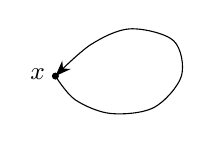
\begin{tikzpicture}[x=0.5mm,y=0.5mm,line cap=round,line join=round,font=\scriptsize]
\node[pt] at (33,-25) {};
\node[inner sep=1pt] at (28.5,-24.5) {\small $x$};
\draw[-{Stealth[length=2mm]}] plot[smooth, tension=0.55] coordinates {(33,-25) (38,-31) (47,-34.5) (58,-33) (65,-25) (63,-16) (52,-13) (42,-17) (33,-25)};
\end{tikzpicture}
\end{document}
